\documentclass{article}
\usepackage{color}
\usepackage{array}
\usepackage{verbatim}
\usepackage{float}
\usepackage{amsmath}
\usepackage{nopageno}
\usepackage{amssymb}
\usepackage{esint}

\usepackage{tikz,tkz-base}
\usetikzlibrary{shapes,decorations,shadows}
\usetikzlibrary{decorations.pathmorphing}
\usetikzlibrary{decorations.shapes}
\usetikzlibrary{fadings}
\usetikzlibrary{patterns}
\usetikzlibrary{calc}
\usetikzlibrary{decorations.text}
\usetikzlibrary{decorations.footprints}
\usetikzlibrary{decorations.fractals}
\usetikzlibrary{shapes.gates.logic.IEC}
\usetikzlibrary{shapes.gates.logic.US}
\usetikzlibrary{fit,chains}
\usetikzlibrary{positioning}
\usetikzlibrary{positioning,calc}
\usepgflibrary{shapes}
\usetikzlibrary{scopes}
\usetikzlibrary{arrows}
\usetikzlibrary{backgrounds}



\definecolor{alizarin}{rgb}{0.82, 0.1, 0.26}
\definecolor{orange}{rgb}{0.9725490,0.7333333,0.5215686}
\definecolor{orange2}{rgb}{0.9921569,0.9215686,0.8588235}
\definecolor{gray2}{rgb}{0.9411765,0.9411765,0.9411765}
\definecolor{cadmiumred}{rgb}{0.89, 0.0, 0.13}
\definecolor{carmine}{rgb}{0.59, 0.0, 0.09}
\definecolor{bostonuniversityred}{rgb}{0.8, 0.0, 0.0}
\tikzset{latent/.style={circle,fill=white,draw=black,inner sep=1pt,
minimum size=30pt, font=\fontsize{10}{10}\selectfont},
obs/.style={latent,fill=gray2},
const/.style={latent, draw=white},
factor/.style={rectangle, fill=black,minimum size=5pt, inner sep=0pt},
>={triangle 45},
squarednodeE/.style={rectangle, draw=black, fill=orange, minimum size=10mm},
squarednodeEd/.style={rectangle, draw=black, fill=orange2, minimum size=10mm},
squarednodeI/.style={rectangle, draw=black, fill=bostonuniversityred!70, minimum size=10mm},
squarednodeId/.style={rectangle, draw=black, fill=bostonuniversityred!20, minimum size=10mm}}

\pgfdeclarelayer{b}
\pgfdeclarelayer{f}
\pgfsetlayers{b,main,f}



\newcommand{\plate}[4]{
\begin{pgfonlayer}{b}
\node (invis#1) [draw, color=white, inner sep=1pt,rectangle,fit=#2] {};
\end{pgfonlayer}\begin{pgfonlayer}{f}
\node (capt#1) [ below left=0 pt of invis#1.south east, xshift=2pt,yshift=1pt]      {\footnotesize{#3}};
\node (#1) [draw,inner sep=1pt, rectangle,fit=(invis#1) (capt#1),#4] {};
\end{pgfonlayer}
}


\begin{document}

\begin{figure}[H]
\begin{center}
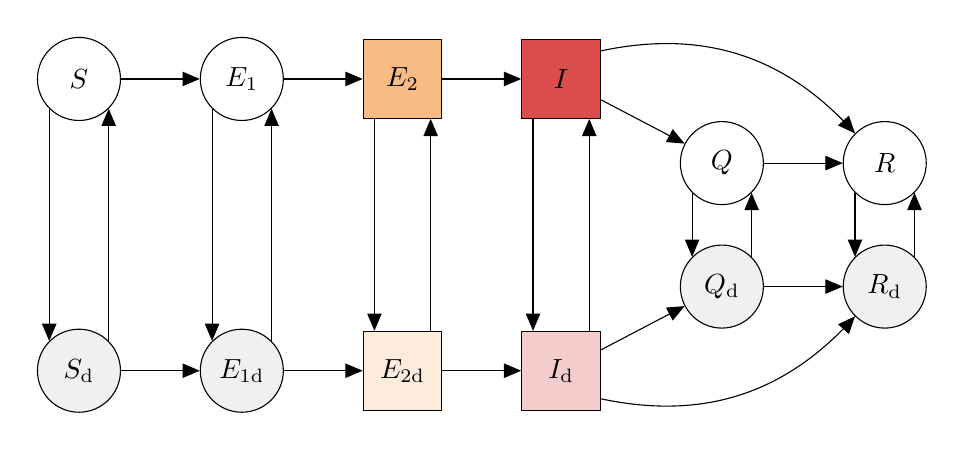
\begin{tikzpicture}
  \matrix[row sep=0mm, column sep=10mm, matrix anchor=mid] (all) {
    \node(S) [latent] {$S$}; & \node(E1) [latent] {$E_1$}; & \node(E2) [squarednodeE] {$E_2$}; & \node(I) [squarednodeI] {$I$}; & & \\
    & & & & \node(Q) [latent] {$Q$}; & \node(R) [latent] {$R$}; \\[5mm] & & & & & \\
    & & & & \node(Qd) [obs] {$Q_\mathrm{d}$}; & \node(Rd) [obs] {$R_\mathrm{d}$}; \\
    \node(Sd) [obs] {$S_\mathrm{d}$}; & \node(E1d) [obs] {$E_{1\mathrm{d}}$}; & \node(E2d) [squarednodeEd] {$E_{2\mathrm{d}}$}; & \node(Id) [squarednodeId] {$I_\mathrm{d}$}; & & \\
  };

\draw
(S)
   edge [->]
(E1);
\draw
(E1)
   edge [->]
(E2);
\draw
(E2)
   edge [->]
(I);
\draw
(I)
   edge [->]
(Q);
\draw
(Q)
   edge [->]
(R);
\draw
(Sd)
   edge [->]
(E1d);
\draw
(E1d)
   edge [->]
(E2d);
\draw
(E2d)
   edge [->]
(Id);
\draw
(Id)
   edge [->]
(Qd);
\draw
(Qd)
   edge [->]
(Rd);
\draw
(S.south west)
   edge [->]
(Sd.north west);
\draw
(Sd.north east)
   edge [->]
(S.south east);
\draw
(E1.south west)
   edge [->]
(E1d.north west);
\draw
(E1d.north east)
   edge [->]
(E1.south east);
\draw
([xshift=+1.5mm]E2.south west)
   edge [->]
([xshift=+1.5mm]E2d.north west);
\draw
([xshift=-1.5mm]E2d.north east)
   edge [->]
([xshift=-1.5mm]E2.south east);
\draw
([xshift=+1.5mm]I.south west)
   edge [->]
([xshift=+1.5mm]Id.north west);
\draw
([xshift=-1.5mm]Id.north east)
   edge [->]
([xshift=-1.5mm]I.south east);
\draw
(Q.south west)
   edge [->]
(Qd.north west);
\draw
(Qd.north east)
   edge [->]
(Q.south east);
\draw
(R.south west)
   edge [->]
(Rd.north west);
\draw
(Rd.north east)
   edge [->]
(R.south east);
\draw
([yshift=-1.5mm]I.north east)
   edge [->,bend left=30]
(R.north west);
\draw
([yshift=1.5mm]Id.south east)
   edge [->,bend right=30]
(Rd.south west);
\end{tikzpicture}
\end{center}
\end{figure}
\end{document}
